\documentclass[12pt,letterpaper]{article}
\input{../../preamble}
\usepackage{fullpage}
\usepackage{multicol}

\begin{document}
\flushleft
\begin{multicols}{2}
\textbf{Math 2554 Exam 4: $\oint 4.6-5.4$ \\
Friday 24 April 2015}

%\hfill
\textbf{Name:  }\underline{\hspace{45ex}} %KEY\hspace{17ex}}

\vspace{.5in}

\end{multicols}

\pagestyle{empty}

\flushleft

\begin{center}\LARGE Calculus I 

Exam 4 \end{center}

\vspace{1.75pc}
Please provide the following data:

\vspace{1.75pc}
Drill Instructor: \underline{\hspace{40ex}}

\vspace{1.75pc}
Drill Time: \underline{\hspace{40ex}}

\vspace{1.75pc}
Student ID or clicker \#: \underline{\hspace{40ex}}

%\vfill
\vspace{3pc}
{\bf Exam Instructions:} You have 50 minutes to complete this exam.  This exam is open resources.  Write on your test which resources you used, and where in the problem you used them.  Justification is required for all problems.  If your answer is wrong, showing more steps can earn you partial credit.  The grading will be \underline{picky} on notation.

%\vspace{2pc}
\vfill
\textbf{Your signature below indicates that you have read this page and agree to follow the Academic Honesty Policies of the University of Arkansas.}  

\vspace{5pc}
Signature: {\bf (1 pt)} \underline{\hspace{91ex}}

%\vfill
\begin{flushright}\Large Good luck!\end{flushright}

% % % % %	
\newpage

\begin{enumerate}[1.]

\item {\bf (5 points)} By visual inspection, locate all points on the graph at which the slope of the tangent line equals the average rate of change of the function over the interval $[-4,4]$.

\vspace{1pc}
\begin{center}
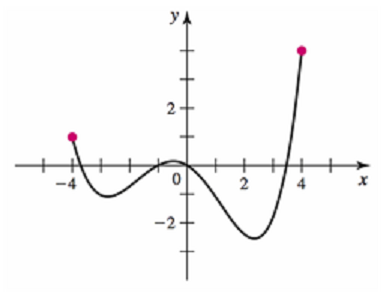
\includegraphics[scale=1.25]{Exam4pic}

\vspace{0.5pc}{\footnotesize from Briggs, et al.}
\end{center}

% % %
\newpage
\item {\bf (3 pts ea)} Suppose
\[\int_1^4f(x)dx=8 \qquad\text{ and }\qquad \int_1^6f(x)dx=5.\]
Evaluate the following integrals:
	
	\begin{enumerate}
	\item $\displaystyle\int_1^4\left(-3f(x)\right)dx$
	
	\vspace{12pc}
	\item $\displaystyle\int_6^412f(x)dx$
	
	\vspace{14pc}
	\item $\displaystyle\int_4^6\left(f(x)+3x\right)dx$
	\end{enumerate}

% % %
\newpage
\item {\bf (6 pts ea)} Evaluate the following limits:
	
	\begin{enumerate}
	%\item $\displaystyle\lim_{x\to 0^+}(\sin x)\sqrt{\frac{1-1}{x}}$
	\item $\displaystyle\lim_{x\to 1^-}(1-x)\tan{\left(\frac{\pi x}{2}\right)}$
	
	\vspace{24pc}
	\item $\displaystyle\lim_{\theta\to \frac{\pi}{2}^-}(\tan{\theta}-\sec{\theta})$
	
	% 
	\newpage
	\item $\displaystyle\lim_{z\to\infty}\left(1+\frac{10}{z^2}\right)^{z^2}$
	\end{enumerate}

% % %
\newpage
\item {\bf (7 points)} Find the point(s) at which the function 
\[f(x)=1-|x|\]
equals its average value on the interval $[-1,1]$.  Then draw the picture of $f(x)$, labelling the points and the average value you computed.
	
% % %
\newpage
\item {\bf (3 pts ea)} Fill in the blanks. %with
	%\begin{itemize}
	%\item right, left, or midpoint	
	%\item a possible interval 
	%\item a value of $n$
	%\end{itemize}
%Note: More than one different answer may work.
	
	\vspace{0.5pc}
	\begin{enumerate}
	\item $\displaystyle\sum_{k=1}^{10}f(1+2k)\cdot 2$ is a right
	%\hspace{1ex}\underline{\hspace{18ex}}\hspace{1ex} 
	Riemann sum for $f$ on the interval $\left[\;\underline{\hspace{5ex}}\;,\;\underline{\hspace{5ex}}\;\right]$
	
	\hspace{8pc}with $n=$ \underline{\hspace{5ex}} .
	
	%
	\vspace{11pc}
	\item $\displaystyle\sum_{k=1}^{4}f\left(\frac{3}{2}+\frac{k}{2}\right)\cdot\frac{1}{2}$ is a midpoint
	%\hspace{1ex}\underline{\hspace{18ex}}\hspace{1ex} 
	Riemann sum for $f$ on the interval $\left[\;\underline{\hspace{5ex}}\;,\;\underline{\hspace{5ex}}\;\right]$
	
	\hspace{8pc}with $n=$ \underline{\hspace{5ex}} .
	
	%
	\vspace{15pc}
	\item $\displaystyle\sum_{k=1}^{5}f(2+k)\cdot 1$ is a left
	%\hspace{1ex}\underline{\hspace{18ex}}\hspace{1ex} 
	Riemann sum for $f$ on the interval $\left[\;\underline{\hspace{5ex}}\;,\;\underline{\hspace{5ex}}\;\right]$
	
	\hspace{8pc}with $n=$ \underline{\hspace{5ex}} .
	\end{enumerate}
	
% % %
\newpage
\item {\bf (4 pts ea)} Evaluate each:

	\vspace{0.5pc}
	\begin{enumerate}
	\item $\displaystyle\int_0^{\ln 8}e^xdx$
	
	\vspace{20pc}
	\item $\dfrac{d}{dx}\displaystyle\int_x^0\frac{dp}{p^2+1}$
	
	%\vspace{12pc}
	\newpage
	\item the net area of the region bounded between the $x$-axis and the function $f(x)=x(x-2)(x-4)$
	
	\vspace{27pc}
	\item $\dfrac{d}{dy}\displaystyle\int_2^{y^3}(t^2+t+1)dt$
	\end{enumerate}	

% % %
\newpage
\item {\bf (10 points)} A mass oscillates up and down on the end of a spring.  Find its position $s$ relative to the equilibrium position if its acceleration is
\[a(t)=\sin{(\pi t)},\]
its initial velocity is $v(0)=3$, and its initial position is $s(0)=0$. 	

\end{enumerate}
\end{document}